% CHAPTER - State of the Art ---------------------

% This section lists the current knowledge in the field of your research question

% Start with some more general aspects and go deeper into the specific research field of your thesis

% Ends with description of knowledge closely related to thesis work
 
% \cite{} vs. \citep{} (citeparentesis)

\chapter{Estado da Arte}
    
    A decomposição de sistemas em módulos é um tópico que começou a ser sistematizado e debatido por \cite{parnas72_decomposing_systems} muito antes da massificação dos sistemas de \textit{software}. Neste seu trabalho, Parnas, pretende demonstrar que a eficiência da modularização de um sistema depende do critério utilizado, não sendo apenas a fragmentação em pequenos módulos o trajeto para o sucesso, mas sim a forma como é feita a escolha do critério de segregação. 
    \todo{dar mais contexto}
    Desta forma, recorre à apresentação e a análise de dois critérios distintos para um caso de estudo: o primeiro focado no fluxo do algoritmo e o segundo na ocultação de informação inerente a cada módulo. Realiza de seguida, uma análise comparativa relativa a propriedades de esforço de desenvolvimento, flexibilidade e compreensibilidade. A análise permite concluir que uma decomposição baseada na ocultação de informação é superior dada a forma como as mudanças são mais localizadas e não obrigam a alterações de \textit{design} que abranjam múltiplos módulos do sistema \cite{parnas72_decomposing_systems}. 
   
    A relevância da decomposição funcional de sistemas inicialmente referida por Parnas, reforçou-se pela necessidade na atualidade em distribuir sistemas complexos por infraestruturas de rede como \textit{web services} e objetos remotos resultante dos esforços em lidar com sistemas de maior dimensão e complexidade \citep{kamimura18_city_analogy}. 
    
    \todo{transição da decomposição para reengenharia de apps monolíticas, info artigo de analogia a cidade}
   
    A decomposição funcional é um dos processos fundamentais na reengenharia de aplicações monolíticas. 


\section{Soluções orientados ao código fonte}

    \todo{introdução}

\subsection{Análise estática}
    
    % Com o intuito de atacar o problema recorrendo a técnicas de análise estática, 
    \cite{mazlami17} propõem no seu trabalho 3 estratégias formais de acoplamento posteriormente processadas segundo algoritmos de \textit{clustering}. As estratégias propostas baseiam-se nas classes da aplicação monolítica e seus meta-dados recolhidos do sistema de versões \textit{Git}. \todo{arranjar esta frase}
    Das estratégias propostas, o acoplamento lógico, baseia-se na premissa que as alterações feitas num monólito são realizadas apenas a um módulo em específico, desta forma, analisa-se o histórico de alterações tendo em conta que as classes que se alteram juntas também deverão estar juntas num micro-serviço. O acoplamento semântico, baseia-se em agrupar classes que têm código sobre as mesmas coisas, ou seja, calculando a similaridade de termos de domínio entre 2 classes poderá obter-se uma medida para identificar quão semanticamente próximas são as classes. Por fim, acoplamento por contribuição, baseado na lei de \cite{conwayslaw}, que indica que a estrutura de \textit{software} representa a estrutura da organização, e como tal, módulos específicos que recebem alterações de um conjunto único de elementos da equipa devem manter-se no mesmo micro-serviço. Sobre cada uma das técnicas de acoplamento, é construído um grafo de dependências que será utilizado para aplicação de algoritmos de \textit{clustering}. 
    
    \todo{terminar}
    
    \cite{kamimura18_city_analogy} seguem uma abordagem semelhante relativamente ao uso de algoritmos de \textit{clustering} para realizar as suas propostas de micro-serviços. A extração das classes é iniciada pela identificação dos \textit{endpoints} da API da aplicação em questão, recorrendo a anotações de \textit{frameworks} específicas (ex.: \textit{@Controller} em \textit{Spring}), que identificam os \textit{endpoints} expostos em APIs REST. Para extração de restante conhecimento, recorre-se também a anotações como o \textit{@Entity} e \textit{@Table} para identificar as classes responsáveis por definir a persistência e tratamento dos dados. O método de \textit{clustering} referido neste trabalho tem como um dos principais objetivos lidar com módulos omnipresentes, ou seja, módulos com um elevado número de relações com outros módulos e presentes numa elevada quantidade de módulos. Proposto por \cite{kobayashi12_feature_gathering_software_clustering}, esta estratégia pretende abordar esse problema por enfraquecer a importância atribuída a módulos com essa particularidade facilitando o processo de \textit{clustering} dos componentes \citep{kobayasi13_sarf}.
    
    % NOTAS SOBRE ARTIGO ACIMA: 
    %  - Não fazem o refactor, só fazem a proposta de extração
    %  - Necessita que as classes contendo os endpoints sejam indicadas inicialmente
    
    
    


\subsection{Análise dinâmica}

    De acordo com \cite{is_cohesion_and_coupling_enough_candela16}, técnicas que processam análise de código baseadas nas suas relações sintáticas, recorrendo a métricas como o acoplamento e coesão ou convenções de nomes, não são suficientes para uma identificação ótima, dado que a relação a nível de código poderá não ser a mesma a nível de funcionalidade \citep{fome_jin_18}. De forma a lidar com esta limitação, \cite{fome_jin_18} propõem o uso como base de trabalho de traços de execução recolhidos durante a execução de determinados casos de testes criados pelo utilizador. Segundo, \cite{execution_traces_expose_behaviour_dit13} os traços de execução recolhidos permitem uma exposição de forma mais precisa do verdadeiro funcionamento do \textit{software}. 
    \todo{completar}
    Na aplicação destes métodos, a qualidade dos testes criados é essencial para garantir que exista uma boa cobertura da funcionalidade do sistema \citep{fome_jin_18}.




\section{Soluções orientadas aos modelos}

    \todo{introdução}
   
   \todo{corrigir 3ª frase} 
   \cite{gysel16_service_cutter} seguem uma abordagem orientada aos modelos, recorrendo a artefactos como modelos de domínio e casos de uso para extrair uma representação de grafo. Às arestas do grafo são adicionados pesos de acordo com um conjunto de critérios tendo em vista identificar \textit{clusters} de componentes, e consequentemente bons candidatos a micro-serviços. Tendo em vista a boa seleção de critérios realizou-se um levantamento de 16 critérios de acoplamento para aplicação dos algoritmos de \textit{clustering}, \textbf{Figura \ref{fig:service_cutter_16}}, destilados de acordo com uma análise da literatura e experiência dos autores.
   
 	\todo{adicionar source da imagem}
	\begin{figure}[h]
     	\begin{center}
     		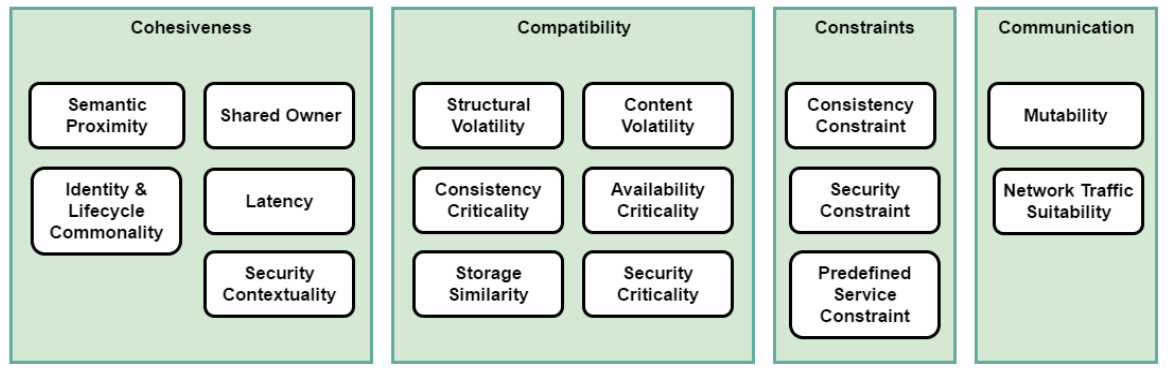
\includegraphics[width=\textwidth]{img/service_cutter_16_criteria.png}
     	\end{center}
     	\caption{Critérios de acoplamento propostos por \cite{gysel16_service_cutter}}
     	\label{fig:service_cutter_16}
 	\end{figure}
   
   Suporta atualmente duas técnicas de \textit{clustering}: \textit{Epidemic Label Propagation} por \cite{leung2009TowardsRC} e o algoritmo de \cite{girvan01_community_structure_cluster}.
   
   No entanto, o \textit{Service Cutter} não tem capacidades de extrair a informação basal necessária para o seu funcionamento de um projeto de \textit{software}, estando altamente dependente dos artefactos de \textit{software} disponibilizados pelo utilizador. Este facto poderá ser limitante em vários sentidos. Em primeiro lugar por se considerar que a documentação é considerada muitas vezes como escassa e desatualizada, em especial nas metodologias atuais Ágeis, que se assentam maioritariamente no \textit{feedback} do utilizador e não em desenvolvimento de documentação. Em segundo lugar, pela necessidade de haver uma correspondência entre os artefactos produzidos e os artefactos esperados pelo \textit{Service Cutter}. \todo{o Service Cutter aceita .json, verificar se a conversão dos modelos típicos é acessível}
   
    % Service Cutter

    % From Monolith to Microservices: A Dataflow-Driven Approach
    % https://ieeexplore.ieee.org/document/8305969


\section{Transição de monólitos para micro-serviços}

\section{\textit{Research gap}}
% sistema que não necessita de um input elevado por parte do utlizador (já existem alguns assim, mas é uma mais valia)
% ServiceCutter
% artigo com os múltiplos tipos de extração do git

% NOTAS: Towards a Framework for generating program source dependence graphs from source code
% Ferramentas como o OPAL, Soot e WALA recorrem a código compilado para a construçao do \textit{program dependence graph}.

% Atlas constrói o grafo apartir de \textit{source code}, mas dada a sua integração com o \textit{Eclipse} é necessário que o código seja compilado e todas as suas dependências estejam resolvidas.  

% Dado o \textit{source code} de um programa, em primeiro lugar ele é convertido para uma gramática que o interpretador por eles proposto perceba.

% De facto é criada a ligação de uma chamada de método para o próprio méotodo.


% \section{Basics/Background/Related work}
% \section{Summary}

